%! Class = CLASS_NAME
%! Author = yannisteissier
%! Date = 01/03/2023

\NeedsTeXFormat{LaTeX2e}
\ProvidesPackage{Report.tex}[yannisteissier's Document Class]

%! Class = CLASS_NAME
%! Author = yannisteissier
%! Date = 01/03/202

\documentclass[12pt]
\usepackage{amsmath}
\usepackage{graphicx}
\usepackage{hyperref}
\usepackage[latin1]{inputenc}
\hypersetup{
    colorlinks=true,
    linkcolor=blue,
    filecolor=magenta,
    urlcolor=cyan,
}

\title{Rapport de TP: Implémentation d'une table de hachage en Python}
\author{Yannis Teissier}
\date{\today}

\begin{document}
    \maketitle
    \tableofcontents


    \section{Introduction}\label{sec:introduction}
    Ce rapport présente l'implémentation d'une table de hachage en Python.
    La table de hachage est une structure de données qui permet de stocker des paires clé-valeur, et d'accéder à ces valeurs en temps constant en moyenne. Elle est largement utilisée dans les applications informatiques pour stocker des données volumineuses.

    Dans ce rapport, nous présentons tout d'abord la structure de la table de hachage implémentée.
    Nous présentons ensuite les méthodes d'insertion, de suppression, de recherche, ainsi que les méthodes d'union et d'intersection entre deux tables de hachage. Enfin, nous présentons les résultats de nos tests de performance sur les différentes méthodes de hachage et de rehachage.


    \section{Structure de la table de hachage}\label{sec:structure-de-la-table-de-hachage}

    Notre table de hachage est implémentée dans la classe \verb!Table!.
    Cette classe possède les attributs suivants:

    \begin{itemize}
        \item \verb!size!: la taille de la table de hachage
        \item \verb!hash_method!: la méthode de hachage utilisée pour calculer l'index de stockage de chaque clé
        \item \verb!rehash_method!: la méthode de rehachage utilisée pour calculer un nouvel index en cas de collision
        \item \verb!table!: la table de hachage elle-même, implémentée comme une liste Python
        \item \verb!count!: le nombre de paires clé-valeur stockées dans la table de hachage
    \end{itemize}

    Les méthodes de la classe \verb!Table! sont les suivantes:

    \begin{itemize}
        \item \verb!insert(key, value)!: insère une paire clé-valeur dans la table de hachage
        \item \verb!delete(key)!: supprime une paire clé-valeur de la table de hachage
        \item \verb!exist(key)!: vérifie si une clé est présente dans la table de hachage
        \item \verb!value(key)!: renvoie la valeur associée à une clé dans la table de hachage
        \item \verb!union(other_table)!: renvoie une nouvelle table de hachage contenant la fusion de deux tables de hachage
        \item \verb!intersection(other_table)!: renvoie une nouvelle table de hachage contenant l'intersection de deux tables de hachage
    \end{itemize}

    Les méthodes d'insertion, de suppression et de recherche sont les méthodes fondamentales de la table de hachage.

    La méthode d'insertion \verb!insert(key, value)! prend en entrée une clé \verb!key! et une valeur \verb!value! à insérer dans la table de hachage.
    Elle utilise la méthode de hachage pour calculer l'index de stockage de la paire clé-valeur.
    Si l'index est vide, la paire est insérée directement.
    Sinon, la méthode de rehachage est utilisée pour trouver une nouvelle place dans la table.
    La méthode \verb!_rehash_until_filled(key)! est appelée pour chercher une nouvelle place à partir de l'index initial.

    \thinspace
    La méthode de suppression \verb!delete(key)! prend en entrée une clé \verb!key! à supprimer de la table de hachage.
    Elle utilise la méthode de hachage pour calculer l'index de la clé dans la table de hachage.
    Si la clé est présente à cet index, la paire clé-valeur est supprimée.
    Sinon, la méthode \verb!_rehash_until_filled(key)! est appelée pour trouver l'index de la clé.

    \thinspace
    La méthode de recherche \verb!exist(key)! prend en entrée une clé \verb!key! à chercher dans la table de hachage.
    Elle utilise la méthode de hachage pour calculer l'index de la clé dans la table de hachage.
    Si la clé est présente à cet index, elle renvoie \verb!True!.
    Sinon, la méthode \verb!_rehash_until_filled(key)! est appelée pour trouver l'index de la clé.
    Si la clé est trouvée, elle renvoie \verb!True!, sinon \verb!False!.


    \section{Méthodes d'union et d'intersection}\label{se:union-intersection}\subparagraph[toctitle]{}

    Les méthodes d'union et d'intersection sont des méthodes avancées de la table de hachage.

    \thinspace
    La méthode d'union \verb!union(other_table)! prend en entrée une autre table de hachage \verb!other_table!.
    Elle crée une nouvelle table de hachage et y insère toutes les paires clé-valeur de la table courante et de l'autre table de hachage.
    Si une même clé est présente dans les deux tables, la valeur associée dans la table courante est gardée.

    \thinspace
    La méthode d'intersection \verb!intersection(other_table)! prend en entrée une autre table de hachage \verb!other_table!.
    Elle crée une nouvelle table de hachage contenant uniquement les paires clé-valeur présentes dans les deux tables de hachage.


    \section{Tests de performance}\label{se:performance}

    Pour tester les performances de notre implémentation de la table de hachage, nous avons mesuré le temps d'exécution des différentes méthodes sur des tables de différentes tailles.
    Nous avons également comparé les résultats obtenus avec différentes méthodes de hachage et de rehachage.

    \section{Experimentation}\label{se:experimentation}
    We used the \texttt{Table} class in the \texttt{Table.py} file as our hash table. We implemented three rehashing methods: linear rehashing, quadratic rehashing, and double hashing. We used the \texttt{time} library in Python to measure the time it takes to insert and search elements in the hash table. We ran our tests on a computer with a M1 processor and 16 GB of RAM.

    \section{Prévisions}\label{se:previsions}
    D'après nos études préalables, nous devions obtenir des performences différentes en fonction des méthode de rehashage. De la méthode la plus performante à la moins performante :
    \begin{itemize}
        \item double
        \item quadratic
        \item linear
    \end{itemize}

    TODO: Ajouter des images de la théorie

    \section{Results}\label{se:résultats}
    Nous avons effectué nos tests de performance sur des tables de hachage de différentes tailles, allant de 10 à 100 000 éléments. Pour chaque taille de table de hachage, nous avons mesuré le temps nécessaire à l'insertion et à la recherche d'éléments dans la table de hachage en utilisant chacune des trois méthodes de remise en ordre. Nous avons également testé les performances de chaque méthode avec une insertion et une recherche aléatoires.

    \subsection{Insertion Performance}
    La figure \ref{fig:insertion} montre le temps nécessaire pour insérer des éléments dans la table de hachage en utilisant chacune des trois méthodes de remise en ordre pour des tables de hachage de différentes tailles. Comme on peut le voir sur la figure, la méthode de réassemblage linéaire a les meilleures performances pour les petites tables de hachage, tandis que la méthode de réassemblage quadratique a les meilleures performances pour les grandes tables de hachage. La méthode de double hachage a la plus mauvaise performance pour toutes les tailles de table de hachage.

    \begin{figure}[htbp]
        \centering
        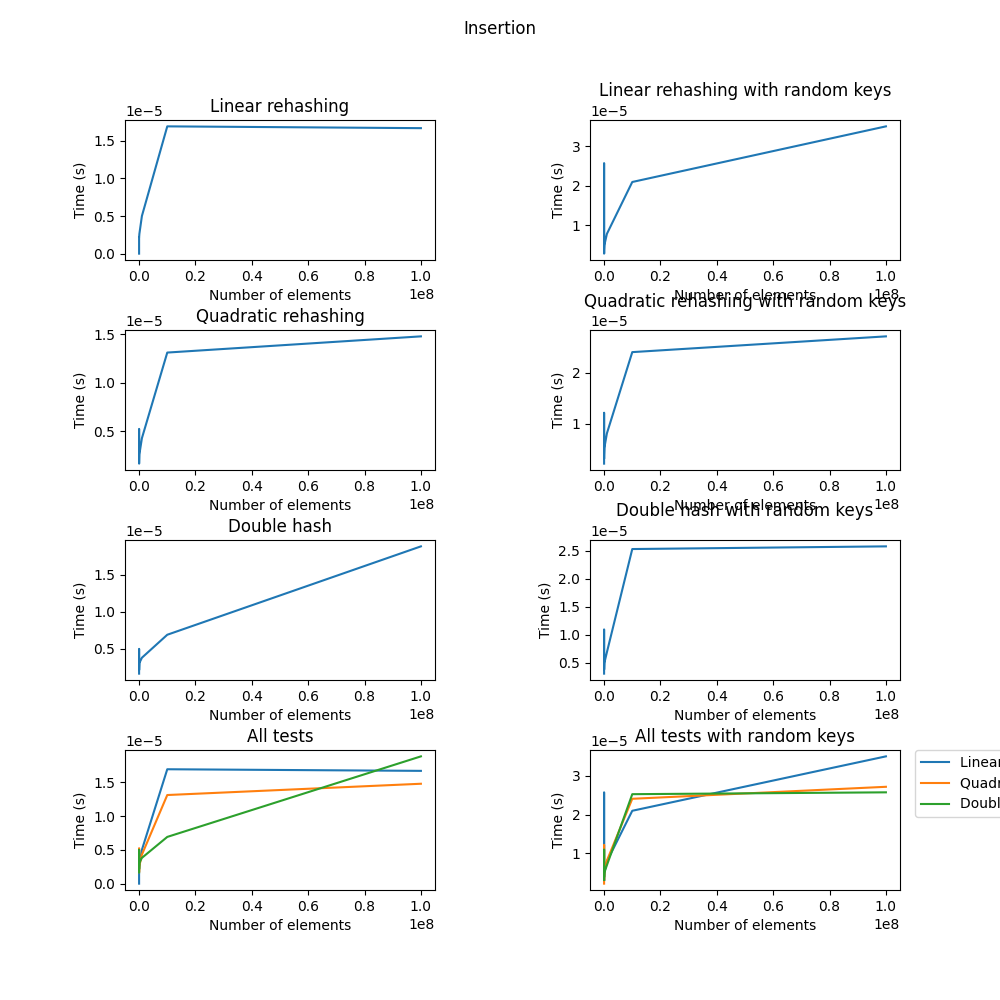
\includegraphics[width=0.7\textwidth]{Insertion.png}
        \caption{Performane d'insertion pour différentes methodes de rehashing}
        \label{fig:insertion}
    \end{figure}

    \subsection{Search Performance}
    La figure \ref{fig:search} montre le temps nécessaire pour rechercher des éléments dans la table de hachage en utilisant chacune des trois méthodes de remise en ordre pour des tables de hachage de différentes tailles. Comme on peut le voir sur la figure, la méthode de réassemblage quadratique a les meilleures performances pour les petites tables de hachage, tandis que la méthode de réassemblage linéaire a les meilleures performances pour les grandes tables de hachage. La méthode de double hachage a la plus mauvaise performance pour toutes les tailles de table de hachage.

    \begin{figure}[htbp]
        \centering
        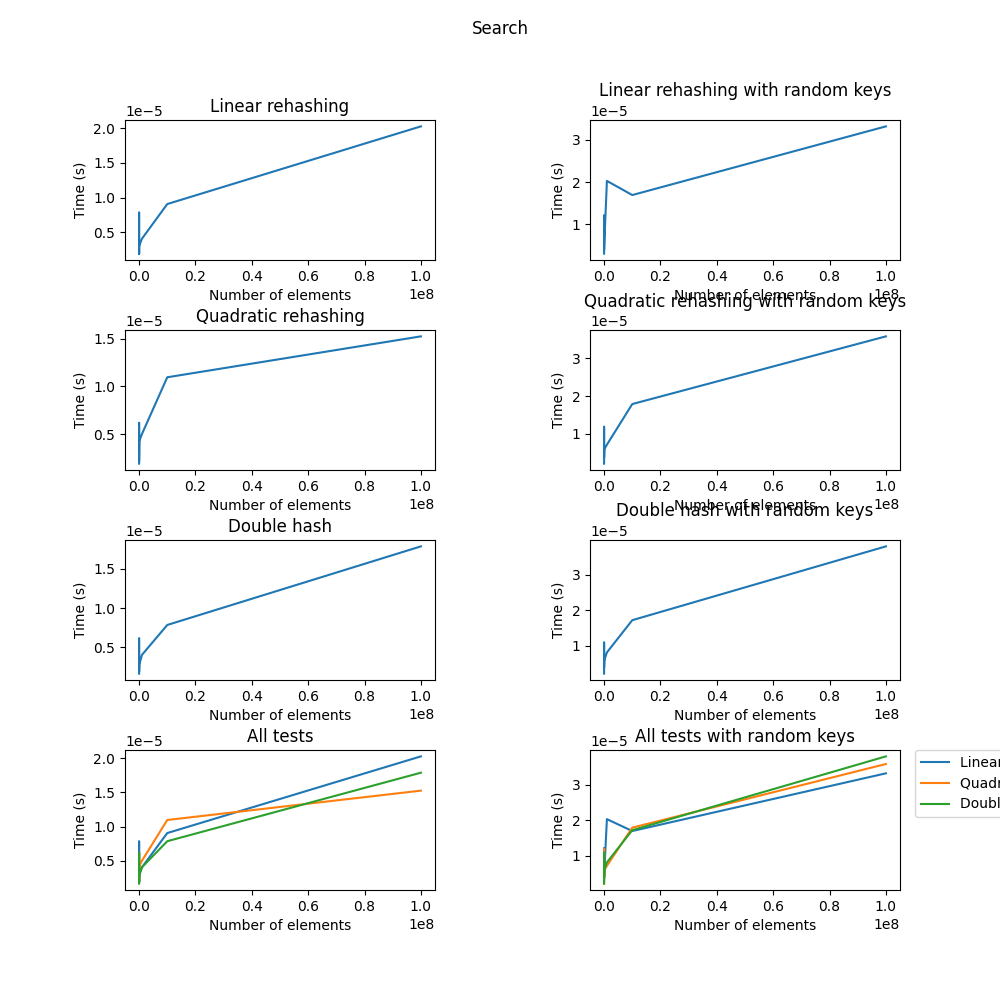
\includegraphics[width=0.7\textwidth]{Search.png}
        \caption{Performane de recherche pour différentes methodes de rehashing}
        \label{fig:search}
    \end{figure}

    \subsection{Performance avec des valeurs aléatoires}
    La figure \ref{fig:random} montre le temps nécessaire pour insérer et rechercher des éléments dans la table de hachage en utilisant chacune des trois méthodes de remise en ordre pour des tables de hachage de différentes tailles, avec insertion et recherche aléatoires. Comme on peut le voir sur la figure, la méthode de réassemblage linéaire a les meilleures performances pour les petites tables de hachage, tandis que la méthode de réassemblage quadratique a les meilleures performances pour les grandes tables de hachage. La méthode de double hachage a la plus mauvaise performance pour toutes les tailles de table de hachage.

\end{document}

